% \thispagestyle{PrimeraPag}
% includeheadfoot, heightrounded, left=1cm, right=1cm, top=1cm, bottom=1cm, headheight=7em, footskip=1.5em]
% \newgeometry{includeheadfoot, heightrounded, left=1cm, right=1cm, top=1cm, bottom=1cm, headheight=7em, footskip=1.5em, showcrop, showframe}
% \savegeometry{Alt}
\thispagestyle{formato-PI}

\renewcommand{\Elaboro}{XXXX}
\renewcommand{\Reviso}{YYYY}
\renewcommand{\Autorizo}{ZZZZ}
\renewcommand{\MayorVer}{3}             % Renovar comando, Versión mayor
\renewcommand{\MenorVer}{0}             % Renovar comando, Versión menor
\renewcommand{\Codigo}{PRO-AC-101}      % Renovar comando, código del documento
\renewcommand{\FechaPub}{2023--01}      % Renovar comando, Fecha de publicación
\renewcommand{\Titulo}{Elaboración y control de documentos} % Renovar comando, Titulo del documento

\section{\Titulo}   % Sección = Titulo definido en la linea anterior\index{Información documentada!tipo!procedimiento!Elaboración y control de documentos}  % Como se encontrará en el indice\index{Procedimientos!Elaboración y control de documentos}                              % Como se encontrará en el indice

\subsection{Objetivo}
Asegurar que los \glspl{documento} del \gls{SGC} se preparan, revisan, aprueban, publican, distribuyen, implementan y administran de acuerdo a lo especificado en este procedimiento.

\subsection{Alcance}
Este procedimiento aplica a todos los documentos generados internamente por cada uno de los departamentos o de fuentes externas y personal involucrado en la elaboración, consulta y actualización de documentos en el \gls{SGC}

\subsection{Terminología y definiciones}\index{Procedimientos!Elaboración y control de documentos!Terminología y definiciones}
\begin{description}
    \item[\glsname{copia-controlada}] \glsdesc{copia-controlada} 
    \item[\glsname{copia-no-controlada}] \glsdesc{copia-no-controlada} 
    % De ahora en delante se usará el comando definido por el usario como \defglo{} para eficientizar el tiempo
    % NOTA: Debe de estar incluido en el archivo del glosario la definición a introducir (Ver linea 242 del template)
    \defglo{documento-interno}
    \defglo{listado-maestro}
    \defglo{procedimiento-estandar}
    \defglo{procedimiento-estandar-de-limpiesza}
    \defglo{instruccion-de-trabajo}
    \defglo{especificacion}
    \defglo{anexo}
    \defglo{formato}
    \defglo{registro}
\end{description}

\subsection{Responsabilidades}\index{Procedimientos!Elaboración y control de documentos!Responsabilidades}
\subsubsection{Aseguramiento de calidad}
\begin{itemize}
    \item Coordina y verifica que se lleve a cabo la actualización en tiempo y forma de los documentos y registros del Sistema de Calidad.
    \item Administra la totalidad de documentos del Sistema de Calidad.
    \item Asigna la numeración correspondiente a los documentos elaborados.
    \item Responsable de la aprobación, revisión y emisión de documentos de acuerdo con su área de responsabilidad.
\end{itemize}

\subsubsection{Gerente de mantenimiento}
\begin{itemize}
    \item Responsable de la elaboración, actualización, revisión, emisión y aplicación de los documentos generados en su área, así como de los documentos del Sistema de Calidad donde tenga injerencia.
\end{itemize}

\subsubsection{Gerente de operaciones}
\begin{itemize}
    \item Responsable de la elaboración, actualización, revisión, emisión y aplicación de los documentos generados en su área, así como de los documentos del Sistema de Calidad donde tenga injerencia.
\end{itemize}

\subsubsection{Jefe de higiene y sanidad}
\begin{itemize}
    \item Responsable de la elaboración, actualización y aplicación de los documentos generados en su área, así como de los documentos del Sistema de Calidad donde tenga injerencia.
\end{itemize}

\subsection{Procedimiento}
\subsubsection{Generación de Documentos} \label{GenDeDoc}
Determinar la necesidad de documentar y validar con el jefe inmediato del área. Identificar el tipo de documento necesario a generar y proceder a documentar y/o generar el documento en base a los siguientes lineamientos:
\paragraph{Estructura}
\subparagraph{Encabezado}
Todos los documentos deben contenerlo y debe incluir:
\begin{itemize}
    \item Logotipo
    \item Título del documento
    \item Código de identificación del documento
    \item Revisión actual del documento
    \item Fecha de emisión
\end{itemize}

\subparagraph{Código}
El código de identificación del documento está formado de la siguiente manera:
La primera parte consta de 1 a 3 letras, las cuales indican el tipo de documento de acuerdo con la \cref{tbl:1.1}

\begin{longtblr}[%
    label = {tbl:1.1},
    caption = {Categorías según el tipo de información documentada},
    ]{%
    width = 0.35\linewidth,
    colspec = {Q[c,m]Q[c,m]},
    row{even} = {Gallery},
    }
    \toprule
        Código & Tipo de documento \\ \midrule
        LM     & Listado Maestro   \\
        PRO    & Procedimiento     \\
        F      & Formatos          \\
        PR     & Programa          \\
        PO     & Política          \\
        RE     & Reglamento        \\
    \bottomrule
\end{longtblr}

La segunda parte consta de dos letras correspondientes al área que genera el documento (no es limitativo), ver \cref{tbl:1.2}

\begin{longtblr}[%
label = {tbl:1.2},
caption = {Categorías según el área operativa},
]{%
width = 0.35\linewidth,
colspec = {Q[c,m]Q[c,m]},
row{even} = {Gallery},
}
\toprule
GE	& Gerencia \\ \midrule
AC	& Aseguramiento de Calidad \\
MA	& Gerencia de Mantenimiento \\
OP	& Gerencia de Operaciones \\
TR	& Departamento Transportes \\
HS	& Departamento Higiene y Sanidad \\
\bottomrule
\end{longtblr}

Los últimos dos dígitos (dos) indican el número consecutivo del documento del área  departamento. Se inicia con el número uno.

\emph{Ejemplo:} 

\begin{center}
PRO-AC-01
\end{center}

\begin{longtblr}[%
label = {tbl:1.3},
caption = {Ejemplo de la codificación de un documento},
]{%
width = 0.35\linewidth,
colspec = {Q[c,m]Q[c,m]},
row{even} = {Gallery},
}
    \toprule
        PRO	& Procedimiento \\ \midrule
        AC 	& Aseguramiento de Calidad \\
        01	& Número de Documento \\ 
    \bottomrule
\end{longtblr}

\subparagraph{Edición}
Indica el número de veces que el documento ha sido modificado y/o adecuado, se inicia con el número que corresponde a la primera emisión.

\subparagraph{Fecha de Publicación}
Corresponde a la fecha en que el documento se elaboró

\subparagraph{Contenido}
Corresponde a la información que contiene el documento y como debe ser presentada.
\begin{enumerate}
    \item \textbf{Objetivo:} Finalidad para la cual fue creado el documento.
    \item \textbf{Alcance:} Áreas o puestos para los cuales es aplicable el documento.
    \item \textbf{Terminología y Definiciones:} Conjunto de términos o palabras propias utilizadas en un procedimiento.
    \item \textbf{Responsabilidades:} Indica los compromisos de los participantes en el desarrollo de un documento.
    \item \textbf{Procedimiento:} Desarrollo de la actividad o proceso a seguir paso a paso.
    \item \textbf{Frecuencia:} Es la frecuencia con la que se debe realizar cada actividad.
    \item \textbf{Documentos Relacionados:} Todos los documentos con relación al procedimiento.
    \item \textbf{Anexos:} Agregados de un trabajo que se incluyen al final del documento y ofrecen información adicional. 
    \item \textbf{Formatos:} Todos los formatos con relación al procedimiento.
    \item \textbf{Historial de modificaciones:} Muestra cuál ha sido el histórico de las modificaciones o adecuaciones que ha tenido el documento. Se establece la revisión anterior, revisión actual, fecha de las revisiones y una descripción de las modificaciones realizadas.
    \item \textbf{Listado de Distribución:} Lista donde se menciona a quien se le ha compartido el procedimiento o documento y cuenta con copia.
\end{enumerate}

\subparagraph{Tipo de letra}
Los documentos se deben desarrollar con base a la estructura del presente documento y deben ser escritos en letra Calibri 12 pt. Los títulos deben ser en negrilla, combinando mayúsculas y minúsculas.

\subparagraph{Numeración}
Inicie el esquema de numeración partiendo del número 1 y según se requiera, desglose el mismo agregando un punto y un decimal, \emph{por ejemplo:} 1, 1.1, 1.1.1. De ser necesario en cada punto utilicé incisos y /o viñetas.

\subparagraph{Revisar el documento elaborado, para asegurar que se cumplen todos los puntos para la estandarización; que incluye el formato, estructura y contenido.}
\subparagraph{Llevar a cabo la ruta de aprobación del documento}
\subparagraph{Si el documento es aprobado proceder a la difusión e implementación del mismo.}
\subparagraph{Los formatos tienen como mínimo (cuando aplique)}
\begin{itemize}
    \item Código 
    \item Revisión
    \item Titulo 
    \item Numero de hojas
    \item Firma de la(s) persona(s) responsable(s) de llenar el registro
    \item Firma de autorización y/o verificación
\end{itemize}

\subparagraph{Los registros son llenados en cada uno de sus espacios, cuando un espacio no es utilizado, por no ser necesario se coloca una línea horizontal o diagonal para cancelarlo.}

\subparagraph{Todos los documentos y registros deben resguardarse de manera que no sufran daño y/o deterioro.}

\subsubsection{Revisión y aprobación de Documentos} \label{RevApDoc}
\begin{enumerate}
\item Si el documento presenta faltas de cumplimiento al presente procedimiento, la persona responsable de la revisión notifica al puesto que generó el documento para que proceda a realizar las modificaciones señaladas y repita las actividades a partir del punto 
\item Si el documento fue aprobado por los involucrados en la ruta de aprobación se procede a su difusión e implementación.
\end{enumerate}

\subsubsection{Distribución, implementación y control de Documentos}
\begin{enumerate}
    \item Los documentos aprobados serán incluidos con la codificación correspondiente en el Listado Maestro de documentos para su control.
    \item Ya liberado el documento (emisión inicial o cambios) el Jefe de Aseguramiento de Calidad realizará las copias y distribuirá el documento de acuerdo a 12 Listado de Distribución.
    \item Cuando se requiera una copia física de los documentos aprobados y vigentes, se realiza una solicitud a Aseguramiento de Calidad, cada copia deberá ser sellada como se indica en la \cref{an1} según corresponda.
    \item Para solicitar  documentos con copia no controlada, se tiene que mandar una solicitud por escrito al Jefe de Aseguramiento de Calidad especificando el motivo de la solicitud.
\end{enumerate}

\subsubsection{Cambios, alta o baja de documento}
\begin{enumerate}
    \item Para realizar cambios, alta o baja de documentos se debe seguir y cumplir los pasos de la \cref{GenDeDoc} al \cref{RevApDoc} Se debe informar a Aseguramiento de Calidad a través del formato O-F-RCP Solicitud de Alta, Baja o Cambio de documentos. \cref{an2}
    \begin{enumerate}
        \item Cambiar el contenido del documento según los cambios necesarios para adecuarlo al  proceso y/o revisar la propuesta de cambio que haga el área solicitante.
        \item Cambiar la revisión de los documentos (Procedimientos, Instructivos o registros).
        \item Llenar el punto 10 del procedimiento, Historial de Cambios, con las especificaciones generales del cambio.
        \item Actualizar el Listado Maestro.
        \item Para finalizar, el Jefe de Aseguramiento de Calidad imprime el documento autorizado y comienza el proceso de distribución y difusión (ver punto 5.3).
    \end{enumerate}
    \item Cuando se realice algún cambio, se debe actualizar el punto 7.0 Historial de Modificaciones del Documento, este punto muestra cual ha sido el histórico de las modificaciones o adecuaciones que ha tenido el documento.
\end{enumerate}

\subsubsection{Control de documentos obsoletos}
\begin{enumerate}
\item Todo documento tiene  1 año de vigencia. Posterior a esta fecha se debe realizar una revisión, para asegurar que la información es actual y corresponde al proceso y/o actividad que se ejecutan.
\item Retire de los puntos de uso los documentos obsoletos que haya distribuido físicamente de acuerdo al listado de distribución y remplace el documento por la revisión vigente para que el personal involucrado siempre tenga la versión actualizada para ejecutar sus actividades; asegure que todos los documentos obsoletos sean retirados y remplazados.
\item Destruya las copias de los documentos obsoletos y destrúyalos conservando un ejemplar que se identificará con la leyenda de DOCUMENTO OBSOLETO (Véase \cref{an-d}) y consérvelos en base a los lineamientos de Control de Registros. (5.1.14).
\end{enumerate}

\subsubsection{Respaldo de la información}
\begin{enumerate}
    \item La documentos electrónicos del Sistema de Calidad es respaldada por el Jefe de Aseguramiento de Calidad con una frecuencia mensual
\end{enumerate}

\subsection{Frecuencia}
\begin{enumerate}
\item Cada vez que sea necesaria la publicación o modificación de algún documento del sistema de calidad.
\end{enumerate}

\subsection{Documentos relacionados}
\begin{itemize}
    \item Todos los documentos y/o procedimientos relacionados al sistema de calidad.
\end{itemize}

\subsection{Formatos}
\begin{itemize}
    \item Formato de cambio de procedimiento \emph{O-F-RCP}
\end{itemize}

\begin{changelog}[simple, sectioncmd=\subsection*,label=changelog-\thesection-\MayorVer.\MenorVer]
	\begin{version}[v=3, date=2023--03--06]
		\item N/A.
	\end{version}

	\begin{version}[v=2, date=2022--03--02]
		\item Cambio de anexos para incluir sellos de control.
	\end{version}

    \begin{version}[v=1, date=2021--09--14]
		\item Origen del documento.
	\end{version}
\end{changelog}

\appendix
\newpage
\section{Sellos para el control documental}

\begin{figure}[h!]
    \centering
    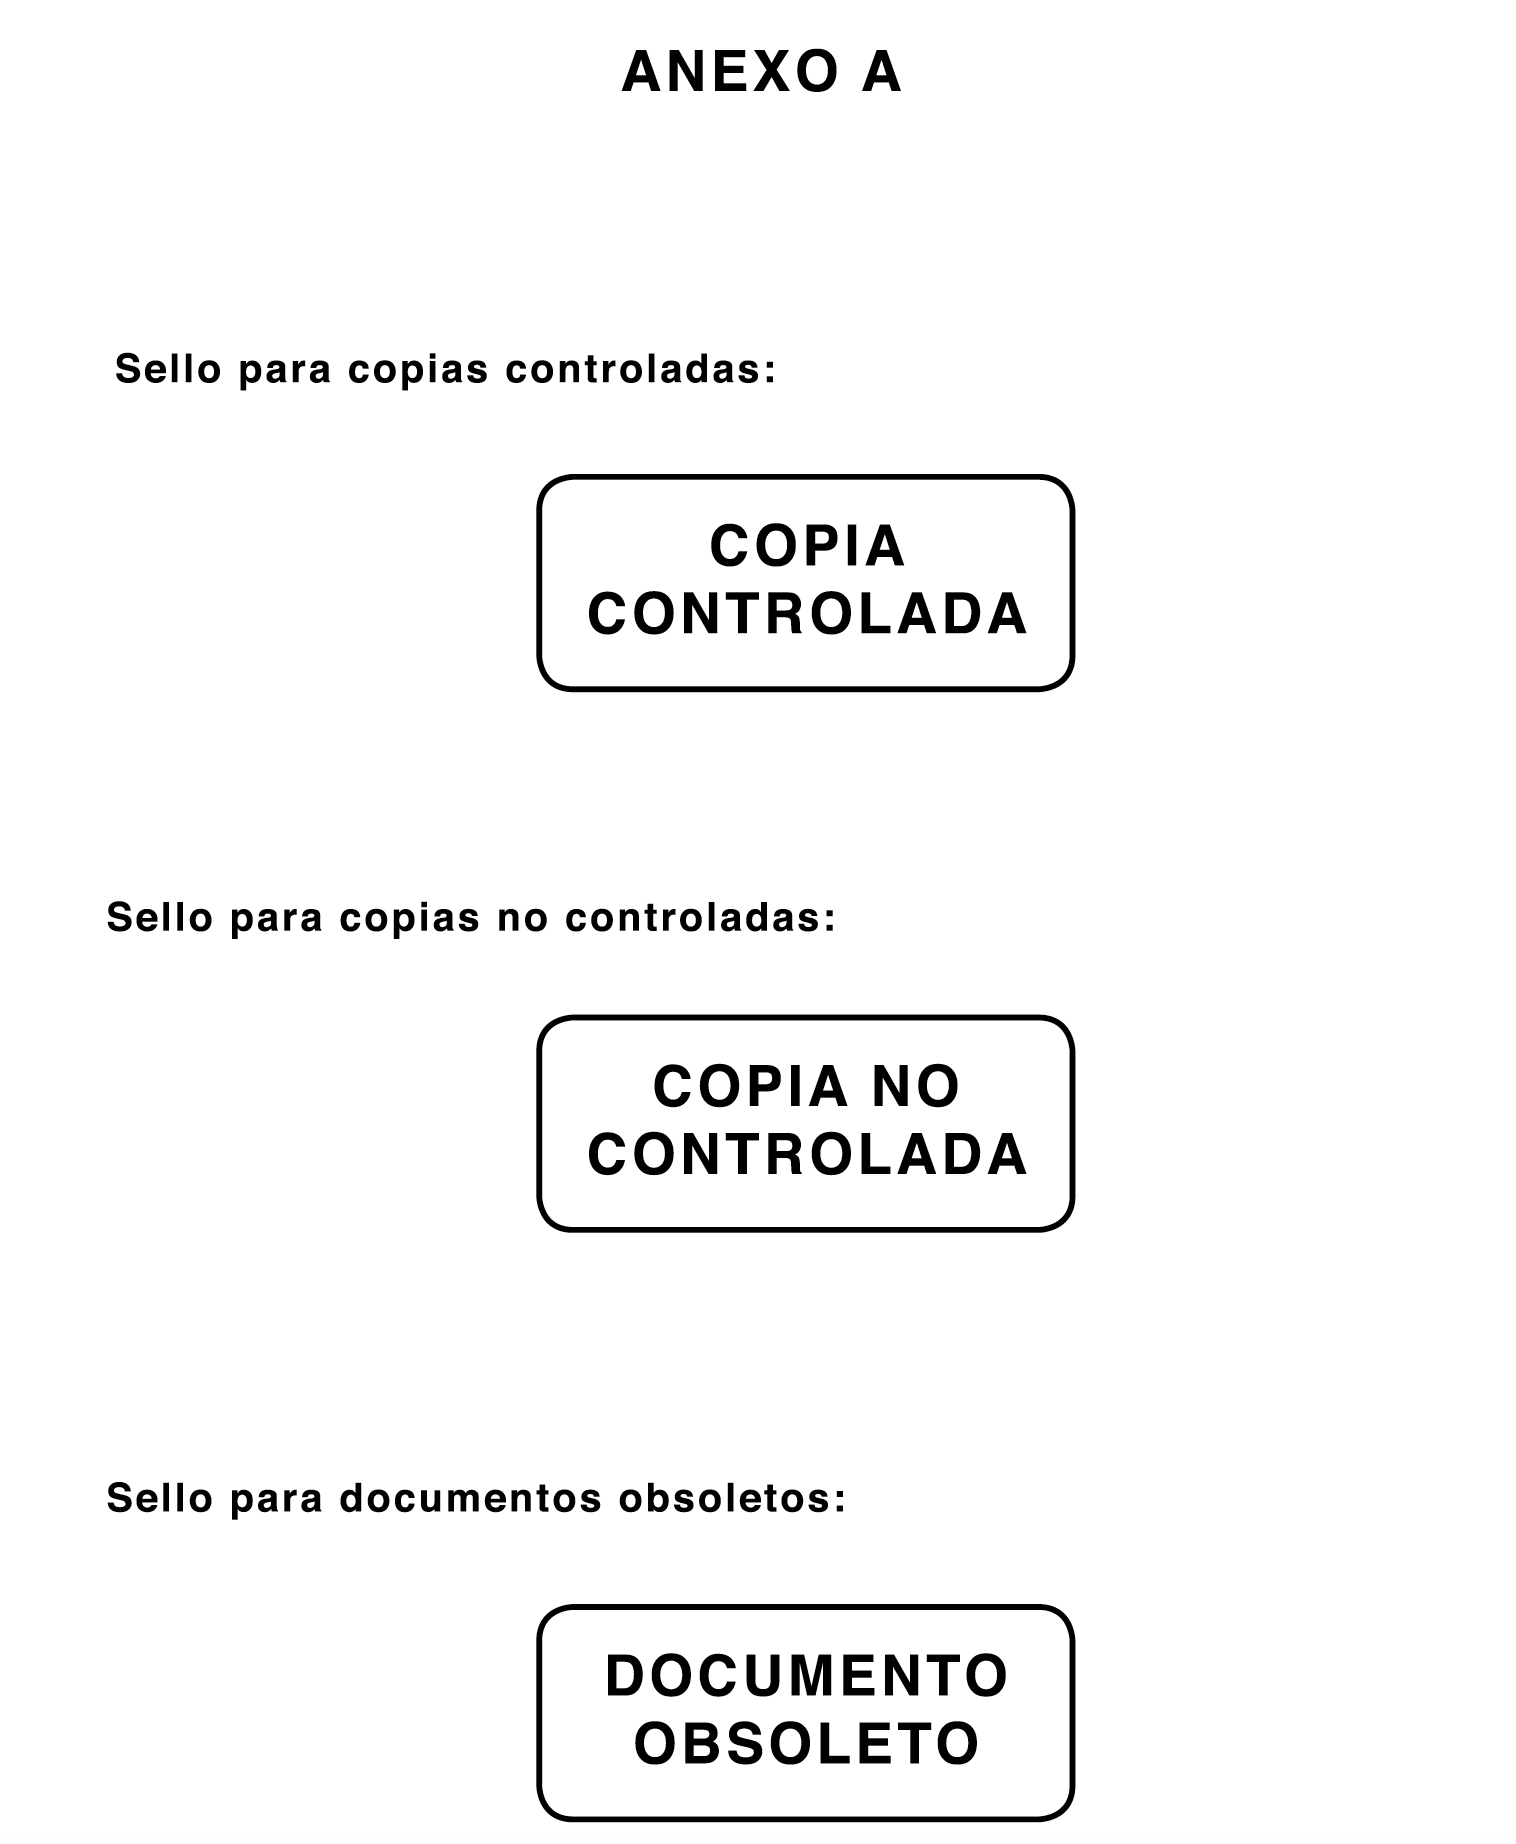
\includegraphics[width=0.5\linewidth]{A1.png}
    \label{an1}
    \caption{Sellos empleados para controlar documentos}
\end{figure}

